%%%
%%% Introduction
%%%
\section{Introduction} % in progress
\label{introduction}
% etliche Leute leiden eines Tages an Rückenschmerzen
% Besonders herausheben: Menschen, die an Rechnern arbeiten
% Problemfeld: degenerative Rückenerkrankungen durch zu lange falsche Haltung
% Unsere Lösung: BodyPose
% Unser Lösungsansatz: webapp die Haltungskorrekturen motiviert
% Unsere Lösung angwandt auf oben beschriebenes Problem
% In Richtung was es sonst noch so gibt -> Überleitung zu related works

\begin{figure}[htpb]
\centering
   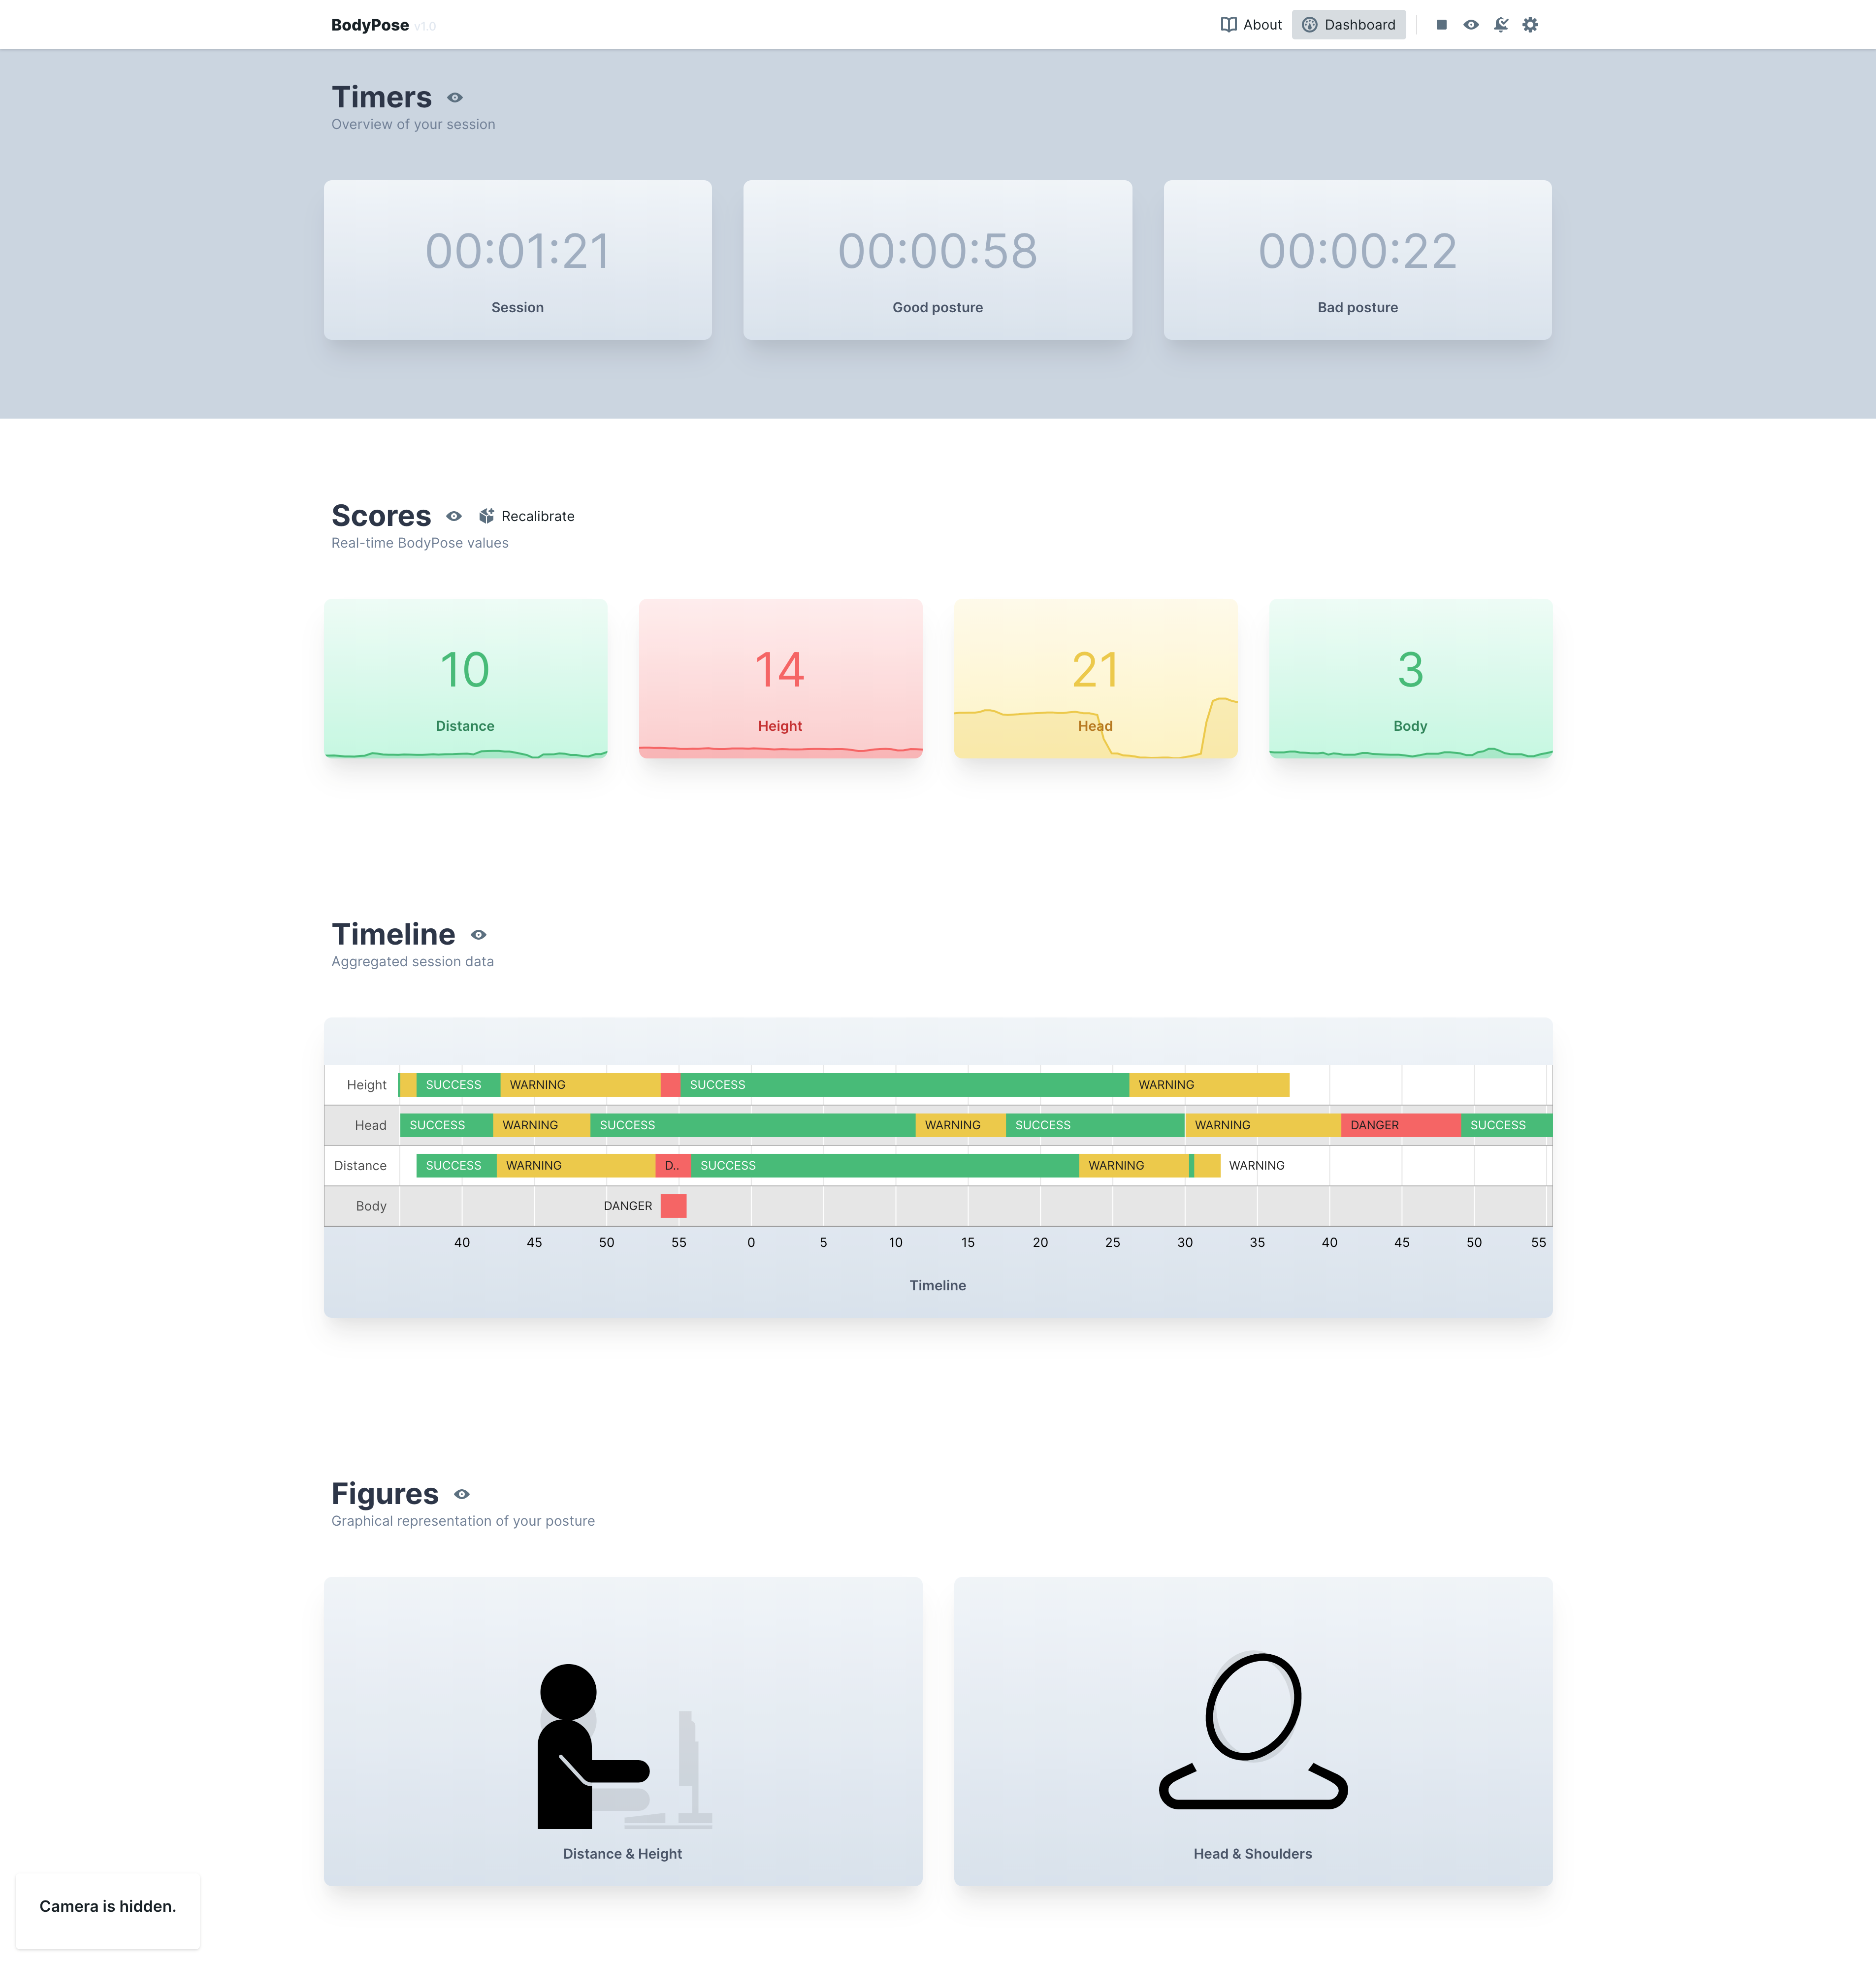
\includegraphics[width=\linewidth]{media/demo.png}
  \caption{Dashboard screen}
  \label{fig:demo-app-screen}
\end{figure}

Suffering from back pain is a severe but common constraint that reduces everyday life quality. With 30\% of European workers suffering from back pain, it tops the list of all reported work-related disorders~\cite{osha2000facts}. Studies regarding this serious medical condition show that 60\% - 90\% of people will suffer from low back disorders at some point in their life~\cite{osha2000facts}. As for 57 \% of all employees in EU the work environment includes working with computers on a daily basis (2019)~\cite{eurostat_comp_use}, it is necessary that precaution tools, as well as education, are provided for employees in order to prevent them from getting back pain. The European Agency for Safety and Health at work states, that "exposure to ergonomic risks factors represents one of the major occupational safety and health problems in the EU today. Repeated exposure to these risks can result in work-related musculoskeletal disorders — one of the most serious and widespread work-related illnesses, which give rise to major cost burden for individuals, businesses and society in general."~\cite{osha2019msd}

Motivated by this severe long-term health threat starting point, we designed the web app BodyPose. While running in the background, it encourages users to maintain or realign their posture. BodyPose observes the user's posture via webcam, which is then recognised by the underlying \textit{PoseNet} model. The data points returned by the model are evaluated by a rule-based system, which triggers notifications to the user in case of misalignment. Users can adjust the sensitivity of the notification threshold to their liking for different body parts independently. BodyPose is designed as a light-weight application, which can be run on various devices supporting a web browser, to allow users to stay flexible within their preferred working devices.

\subsection*{Contribution}
Our approach offers an easily accessible, open-source motivational solution for preventing back and neck pain related to office work and other forms of prolonged sitting in front of a computer. Our solution has minimal setup requirements: Anyone with a computer, a working internet connection and a webcam can use our web-based application. While the rule-based pose evaluation system employed in our approach draws inspiration from previous related work, our approach is - to the best of our knowledge - the first and only one to employ the publicly available Tensorflow.js~\footnote{TensorFlow for Javascript} \textit{PoseNet} model for this health-related use. 

%Brauchbarer Übergang zu related works?

%%%
%%% Related Work
%%%
\section{Related Work} % in progress
\label{related-work}
The idea of designing a system that can monitor and evaluate the upper body posture of a user is not novel. Previous work in academia emphasises the risks of bad posture habits, and previous approaches to a solution for this problem can be found not only in academia but also in the form of a commercial product line. While the goal of helping users to maintain a healthy body posture is common to all of these approaches, including ours, there are also some noteworthy differences, which will be mentioned in the following section. 
\subsection{Computer-related musculoskeletal disorders}
Several scientific publications show that excessive computer usage can cause musculoskeletal symptoms such as neck, shoulder and back pain. \citeauthor{hakala2006frequent} \cite{hakala2006frequent} argued that the increase of these symptoms in the 1990s and 2000 correlate with the increase of using computers.
Regarding a study conducted by \citeauthor{fang2007workers} \cite{fang2007workers}, one-third of missed workdays in US workplaces were due to musculoskeletal disorders. There is evidence that the seated posture applied when working with computers correlates with such disorders\cite{gerr2004epidemiology}. Another key contributor to musculoskeletal disorders in the office workplace is that computers are not only used for prolonged periods but also on a daily basis\cite{gerr2004epidemiology,chang2007daily}. A study by \citeauthor{chang2007daily} conducted with 27 undergraduate students  showed that using computers more than three hours significantly increased the number of musculoskeletal disorders reported by those students.

\subsection{Physiological recommendations}
There are a number of recommendations on how to maintain healthy body postures in order to prevent musculoskeletal disorders. Physiotherapists report that a proper spinal curvature is essential to prevent back pain. However, the exact characteristics of this curvature seem to vary from country to country, making clear recommendations difficult\cite{o2012physiotherapists}. An orthopaedist we contacted during our research phase argued that even a small misalignment of head or shoulders in the form of slouching leads to musculoskeletal disorders when the corresponding posture is held for a longer period. Multiple workspace ergonomics recommendations also state the importance of proper sitting height and distance, such as in \cite{website:muckenthaler_ergonomie}. Based on this information, we derived our four posture measurements (head tilting, shoulder tilting, sitting height, sitting distance). We explain these measures more detailed in \autoref{rulebased}.

\subsection{Posture detection in prior work}
In order to detect poor posture behaviours, different techniques have been applied in prior work. \citeauthor{demmans2007posture} \cite{demmans2007posture} used FLX-01 Flex Sensors to measure forward and backward neck angles. The commercial product line \textit{Upright Go}~\footnote{\href{https://www.uprightpose.com/}https://www.uprightpose.com/} relies on an external sensor appended to the neck and offers apps for iOS and Android devices, as well as a desktop app for Mac~\footnote{In contrast to most of the approaches in academia.}. Some authors in academia experimented with novel sensors such as chair sensors or cloth sensors \cite{bibbo2019sitting,cha2017patient,zhang2019architecture}. In \cite{paliyawan2014prolonged},\cite{paliyawan2014office} and \cite{clark2012validity}, the authors used three-dimensional input (including depth information) from a Microsoft Kinect device to detect body posture with high accuracy with the goal of preventing office worker syndrome. \citeauthor{estrada2017sitting}~ \cite{estrada2017sitting} utilised a conventional webcam in combination with accelerometers from smartphones attached to the back of a sitting user to measure spinal posture, as well as head and shoulders posture. \citeauthor{tanaka2015nekoze} ~\cite{tanaka2015nekoze} focused on head posture not only when using computers, but also smartphones: While a front-facing camera is used for the computer setting, the smartphone use-case employs the accelerometer of smart glasses to estimate the head angle. \citeauthor{jaimes2005sit} ~\cite{jaimes2005sit} used camera and microphone input to monitor not only upper body posture but also user activities (such as reading, stretching, talking on the phone). Their posture recognition is based on using geometric features extracted from the input image. \citeauthor{lintila2016development} ~\cite{lintila2016development} used only a front-facing webcam to detect bad posture. However, they also worked with a test setup including three cameras (for front-, back- and side-view) in order to record experiments and validate their method with the help of an external expert observer (a physiotherapist). Their proposed measurement system could detect 25 \% of the bad posture events the expert observer detected.

% \begin{itemize}
% \item Estrada et al.: Sitting posture recognition for computer users using smartphones and a web camera\cite{estrada2017sitting} $\rightarrow$ Measuring spinal posture and head/shoulders posture using accelerometers from smartphones front camera.
% \item Paliyawan et al:
% Prolonged sitting detection for office workers syndrome prevention using kinect\cite{paliyawan2014prolonged}
% Office workers syndrome monitoring using Kinect\cite{paliyawan2014office} $\rightarrow $  Posture recognition using kinect
% \item Kinect gives high accuracy\cite{clark2012validity}
% \item Tanaka et al.: Nekoze! - monitoring and detecting head posture while working with laptop and mobile phone\cite{tanaka2015nekoze} $\rightarrow$ Laptop based system using the front-facing camera, mobile system using a smart class prototype
% \item Jaimes et al. Webcam but using geometric features of the user's silhuette\cite{jaimes2005sit}
%\item Lintila et al: Development of computer vision-based face tracking measurement for sitting ergonomics\cite{lintila2016development} -> Used 3 cameras (front, back, side) to recognize bad posture. Also, a physiotherapist analysed bad posture. Using just head movement the system 25 percent of bad events that physiotherapist detected compared to
% \end{itemize}

\subsection{Influencing user behaviour and giving feedback}
Our work focuses on bad posture detection in everyday office workspace environments. Reminding the user to keep a healthy posture seems essential, but in doing so, it should disrupt the user's work as little as possible. \citeauthor{haller2011finding} \cite{haller2011finding} analysed different feedback techniques on body posture regarding the impact on a user's workflow and productivity. They used graphical feedback in the form of on-screen notifications, physical feedback in the form of a bending toy flower representing the user's posture and vibrotactile feedback in the form of force feedback using video game controllers. While the graphical feedback appeared to be the least interruptive, it was also more likely to be ignored compared to physical feedback\cite{haller2011finding}. For our work, we decided to use graphical feedback, as it seemed the most feasible option to us. However, the idea of the physical feedback used in the study finds application in the form of a graphical representation that we describe more detailed in \autoref{user_interface}.

Research has also been conducted on how computers can be used as a persuasive technology that impacts the user's behaviour\cite{fogg1998persuasive}.
A study by \citeauthor{duffy2013measuring} \cite{duffy2013measuring} compared different feedback versions and measured the effect on persuading the user to reduce bad body posture behaviours. Three different feedback types were used: Dimming the screen's brightness as soon as a bad posture was detected, an hourly pop-up message informing the user with an overview of the time spent in a bad posture and an hourly pop up with motivational messages\cite{duffy2013measuring}.
Screen dimming performed best, arguably due to being the only feedback type supplied instantly, which created a "cause-effect relationship between the subjects and the computer"\cite{duffy2013measuring}. The work by \citeauthor{jaimes2005sit} already mentioned above also used real-time feedback to inform the user about poor posture. These findings encouraged us to use instant feedback in the form of browser notifications, as well as utilising timers for our dashboard. \autoref{rulebased} and  \autoref{user_interface} offer a more detailed explanation of our feedback system.

%Our approach offers a free, web-based application that relies solely on input from a simple webcam.  Thus, it is easily accessible to anyone with a PC/laptop, webcam and browser.

\section{Technology} % in progress
In the following, we will give an overview of the technology used in our approach. First, we will discuss the different components of our architecture and how they work together in evaluating body posture and giving feedback to the user. Additionally, we will give an overview of the user interface.

\subsection{Components} % in progress
Our architecture is composed of two main components: First, we make use of the TensorFlow.js \textit{PoseNet} model to identify key points on the upper body of a user from webcam images. Specific key points are then used as input by the second main component, a rule-based system that evaluates the upper body posture and gives feedback according to the preferences set by the user. In the following, we will discuss these main components in detail.

\subsection*{PoseNet}
Pose estimation, the first step in our pose evaluation pipeline, "refers to computer vision techniques that detect human figures in images and videos, so that one could determine, for example, where someone’s elbow shows up in an image"~\cite{tflite_pose_estimation}. For this task, we employ the publicly available \textit{PoseNet}, a "vision model that can be used to estimate the pose of a person in an image or video by estimating where key body joints are"~\cite{tflite_pose_estimation}, implemented in TensorFlow.js. These key points include facial landmarks (nose, eyes and ears), shoulders, elbows, wrists, hip, knees and ankles. To detect them and their position (x and y coordinates) in an RGB image, \textit{PoseNet} first feeds this input RGB image through a convolutional neural network and then applies a pose-decoding algorithm to the output of the network in order to return poses, pose confidence scores~\footnote{"Determines the overall confidence in the estimation of a pose. It ranges between 0.0 and 1.0."~\cite{tf_js_pose_estimation}}, keypoint positions, and keypoint confidence scores~\footnote{"Determines the confidence that an estimated keypoint position is accurate. It ranges between 0.0 and 1.0."~\cite{tf_js_pose_estimation}}. We feed an input image to the model every 10 ms.

There are several options and parameters to tune the accuracy and performance of the model. The first of these options is the choice of network architecture: either a lightweight and thus fast \textit{MobileNetV1} architecture can be employed, or a more accurate but slower \textit{ResNet50} architecture. As one of our aims in designing our application is to be resource-efficient regarding required hardware, as well as battery-life, we employ the \textit{MobileNetV1} architecture. 
The second option is the choice between two variants of the pose-decoding algorithm: multi-pose decoding, which can be used to detect poses of multiple persons in an image, and single-pose decoding, which can only detect one pose in an image and thus requires the input image to include only one person in order to function correctly. Furthermore, minimum confidence values, ranging from 0.0 to 1.0, can be set both for pose detection and keypoint detection, in order to ignore poses or keypoints with a confidence value below the respective minimum value. More technical details on the pose-decoding algorithm are discussed in \cite{tf_js_pose_estimation}, \cite{pap2017accurate} and \cite{pap2018personlab}.
We use the multi-pose algorithm, but restrict it to detecting only one pose. Although the single-pose algorithm is considered faster and simpler\cite{tf_js_pose_estimation}, we achieved better results with this setting. However, this also puts a limitation on the use of our application: when there is more than one person included in an input image, the application will not be able to return reliable results regarding the quality of the body posture. Regarding the minimum confidence values, using a value of 0.1 for both pose and keypoint detection yielded satisfactory results.
Further options include the output stride of the convolutional neural network~\footnote{Choice between 8, 16 and 32. Higher output stride results in faster performance but lower accuracy.~\cite{tf_js_pose_estimation}}, a multiplier value determining the number of channels of all \textit{MobileNetV1} convolution operations~\footnote{"Can be one of 1.01, 1.0, 0.75, or 0.50 [\dots]. The larger the value, the larger the size of the layers, and the more accurate the model at the cost of speed."~\cite{posenet_github}}, the number of bytes used in weight quantization~\footnote{Options are no quantization, two bytes per float, and one byte per float. The lower the number of bytes, the lower the model size and accuracy.~\cite{posenet_github}}, and whether to flip the input image horizontally~\footnote{"Should be set to true for videos where the video is by default flipped horizontally (i.e. a webcam), and [\dots] poses [should] be returned in the proper orientation."~\cite{tf_js_pose_estimation}}.
Regarding the trade-off between speed and accuracy, we achieved best results with an output stride of 16, a multiplier value of 0.75 and no weight quantization. We also flipped the input image horizontally, since BodyPose is intended to be used with a webcam.

\subsection*{Rule-based system}
\label{rulebased}
The second step in our pose evaluation pipeline is a rule-based system that evaluates the estimated pose (as returned by \textit{PoseNet}) according to user-defined thresholds and settings. In order to give the user detailed feedback, we refrain from evaluating the pose as a whole. Instead, we evaluate four categories: alignment of the head/neck, alignment of shoulders, sitting height and distance to screen. The measurement and evaluation of these four categories are based on the following input: the current keypoints detected for eyes and shoulders of a user (as returned by the \textit{PoseNet} model), as well as keypoint data gathered at the beginning of a session by a calibration phase. 

The current keypoints are used to determine the inclination angle of head/neck and shoulders as a proxy measurement for the misalignment of these body parts. However, due to the aforementioned trade-off between speed and accuracy of the \textit{PoseNet} model, the coordinates of the detected keypoints tend to unreliably "jump" between pose estimations of successive frames. To counteract this and improve robustness, we accumulate keypoint data over a user-specified time window and calculate the median separately for each coordinate (x, y) of each keypoint over the specified time window. As an alternative measurement of central tendency, calculating the mean instead of the median is offered as an option to the user. However, since we achieved the best results in counteracting these outlier "jumps" with the median calculation, it is used by default.

For evaluating sitting height and distance to the screen, the aforementioned calibration phase is necessary (during which keypoint data is collected in the same manner as above, by aggregating values over a time window). This is due to the following reasons: we can measure sitting height by taking the y coordinates of key points, but to evaluate whether the height has decreased or increased, we need a reference point to compare to. The y coordinates of keypoints saved during calibration serve as these reference points. Consequently, we can detect slouching under the assumption that it is connected with a decreasing sitting height. Additionally, since there is no depth information in the input images, there is no direct way of measuring the distance to the screen/camera. Thus, we approximate it under the following assumption: Given the distances between the left and right shoulder and eye key points at the time of calibration, we can compare these distances to those currently measured. Should the current distances be bigger as those during calibration, we can infer that the user has moved more closely to the screen and vice versa.

Since there is no one-size-fits-all solution for evaluating an upper body posture, we implemented several thresholds and settings that can be changed by the user to fit situation and needs. First, the user can specify thresholds for the absolute inclination angle of both head/neck and shoulders (in degrees), determining what absolute angle should be considered a bad posture. Similar threshold values exist for detecting inadequate sitting height and distance to screen, although not measured in degree, but on a scale ranging from 0 to 100. Since misalignment or wrong distance to screen/sitting height only have a negative health effect when remaining in this position for a certain amount of time, we also implemented a threshold that determines how long a specific value (such as inclination angle of head/neck) must be above its threshold value (without interruption) before the user is notified about the bad posture connected to this value. 

Default threshold values and settings are as follows: 
\begin{itemize}
    \item Threshold of head angle (in degrees): 8
    \item Threshold of shoulder angle (in degrees): 12
    \item Threshold of distance to screen: 20
    \item Threshold of height variance: 10
    \item Time frame of one epoch (in ticks)~\footnote{An epoch defines the window size over which median/mean are calculated. A tick refers to one input image being fed through the \textit{PoseNet} model.}: 100
    \item Time until bad posture triggers notification (in seconds): 10
\end{itemize}


\subsection{User Interface}
\label{user_interface}
When visiting the BodyPose webpage, users will first be directed to an About page, where they can read a short text about the aim of the application (improving body posture habits), as well as a short manual on how to correctly calibrate and use the application. From the About page, users can continue to the dashboard, shown in \autoref{fig:demo-app-screen}, (i.e. the main view of our application) by clicking on the corresponding button at the upper right of the page. When opening the dashboard, users are first asked to calibrate BodyPose before they can start using the application. By clicking on the corresponding button to start the calibration, a popup window is opened. In this window, users are asked to sit straight and place themselves at their usual distance to the screen while being able to see the current camera view. By clicking on the \textit{Calibrate} button, a timer counting down from three gives users enough time to make last adjustments to their position. When the countdown reaches zero, the detected pose will become visible to the user in the current camera view and keypoint data will be gathered and saved for later use. 

After the calibration is finished, users gain access to the full functionality of the Dashboard. In this view, they can monitor information regarding their body posture. This information is divided into multiple sections: First, the \textit{Timers} section gives users an overview of how long their current session has been running and how much of that time they spent maintaining a good or bad pose. Second, the \textit{Scores} section lets users monitor real-time values of the four measurement categories: distance to screen, sitting height, and inclination angles for both head and body (i.e. shoulders). For each measurement, a corresponding box not only shows the real-time numeric values but also changes colour according to the current state of the respective measurement: As long as no threshold value is crossed, boxes remain green to signalise good posture. As soon as a threshold value is crossed, the corresponding box switches to orange to warn the user about a potentially bad posture. Only when this potentially bad posture is held for the user-defined period will the box change to red to indicate the danger of a bad posture (when held for too long).
The third section, \textit{Timeline}, gives users an overview of their aggregated session data: For each of the four measurement categories (distance, height, angle of head, angle of body), a separate (horizontal) timeline will be shown to the user, highlighting phases with their corresponding colour (green for success, orange for warning, and red for danger). 
The fourth and last section, \textit{Figures}, shows users two animated graphical representations of their posture: One representation shows a simplified side view of a user sitting in front of a PC and animates distance to screen and sitting height according to the currently detected pose. The other representation shows a simplified front view of a user, with two distinct animated parts (head and shoulders) representing the inclination angle of the respective body parts.

\begin{figure*}[htpb]
\centering
  \subcaptionbox{Short-term motivation (Likert scale)\label{fig:us-gs-shortterm}}{
    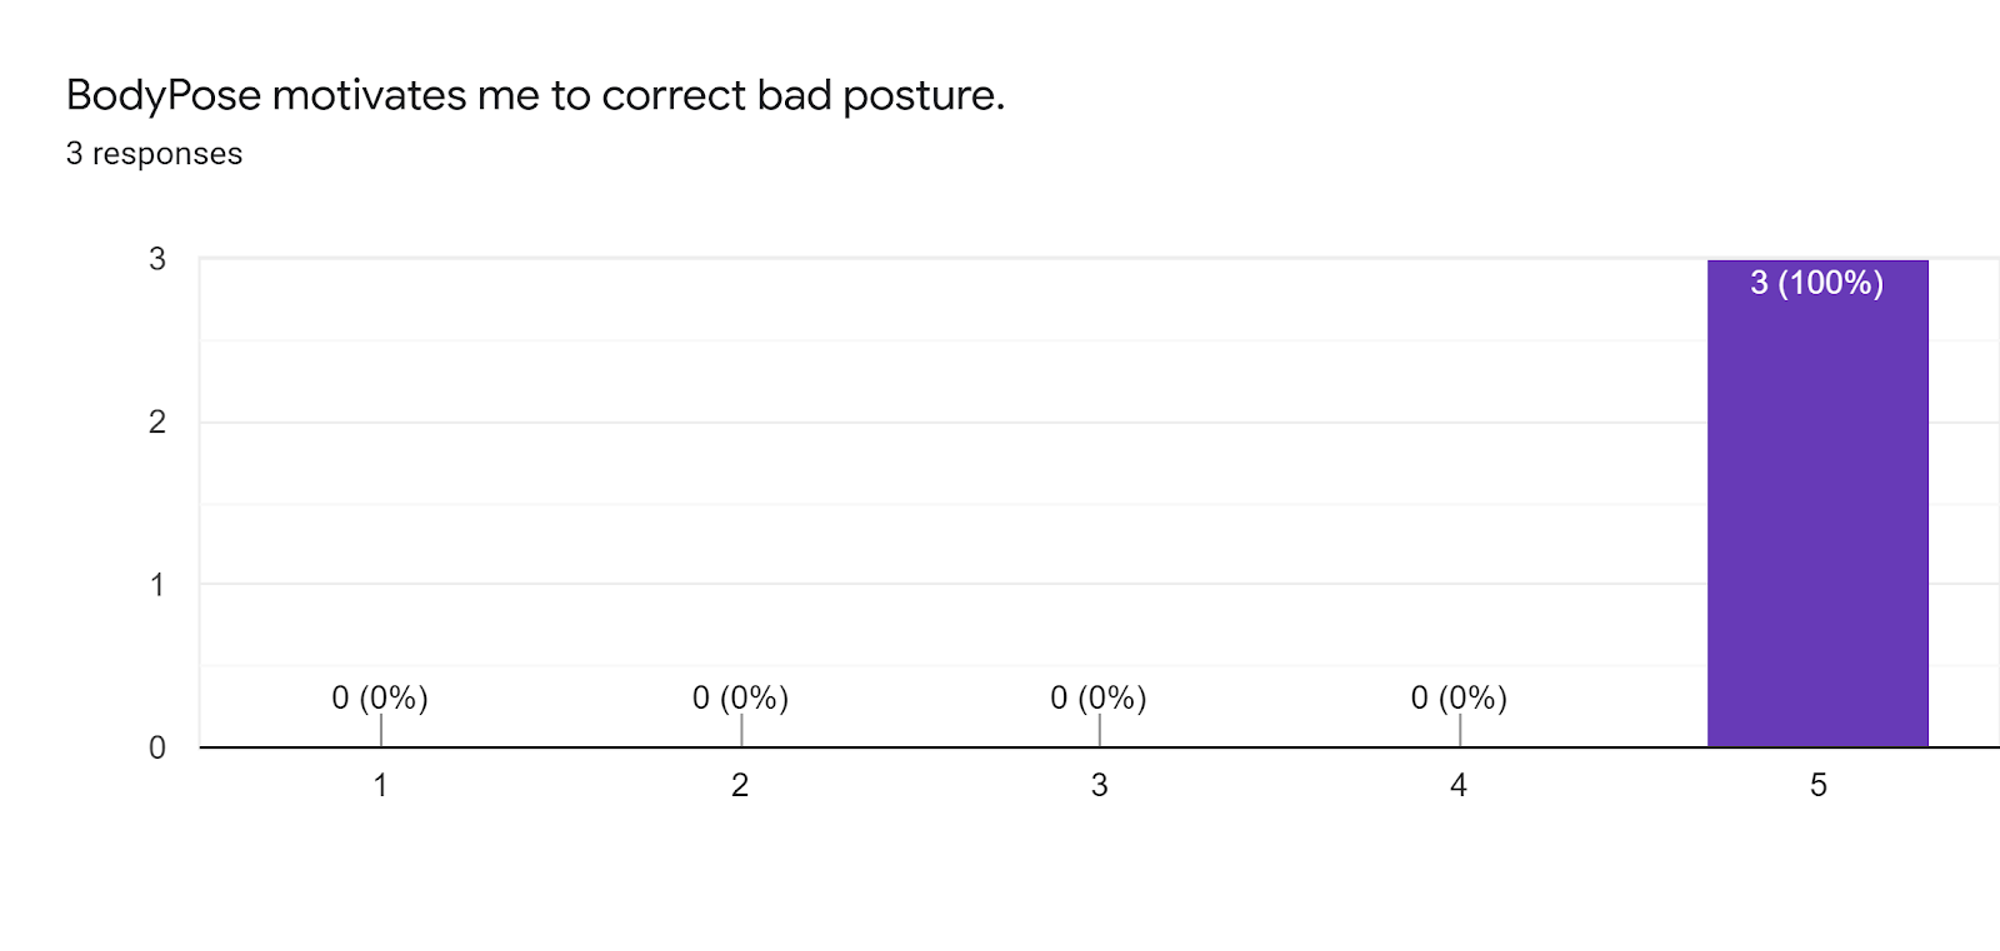
\includegraphics[width=0.32\textwidth]{media/us-gs-shortterm-motivation-results-eng.png}  
  }
  \subcaptionbox{Long-term motivation (Likert scale)\label{fig:us-gs-longterm}}{
    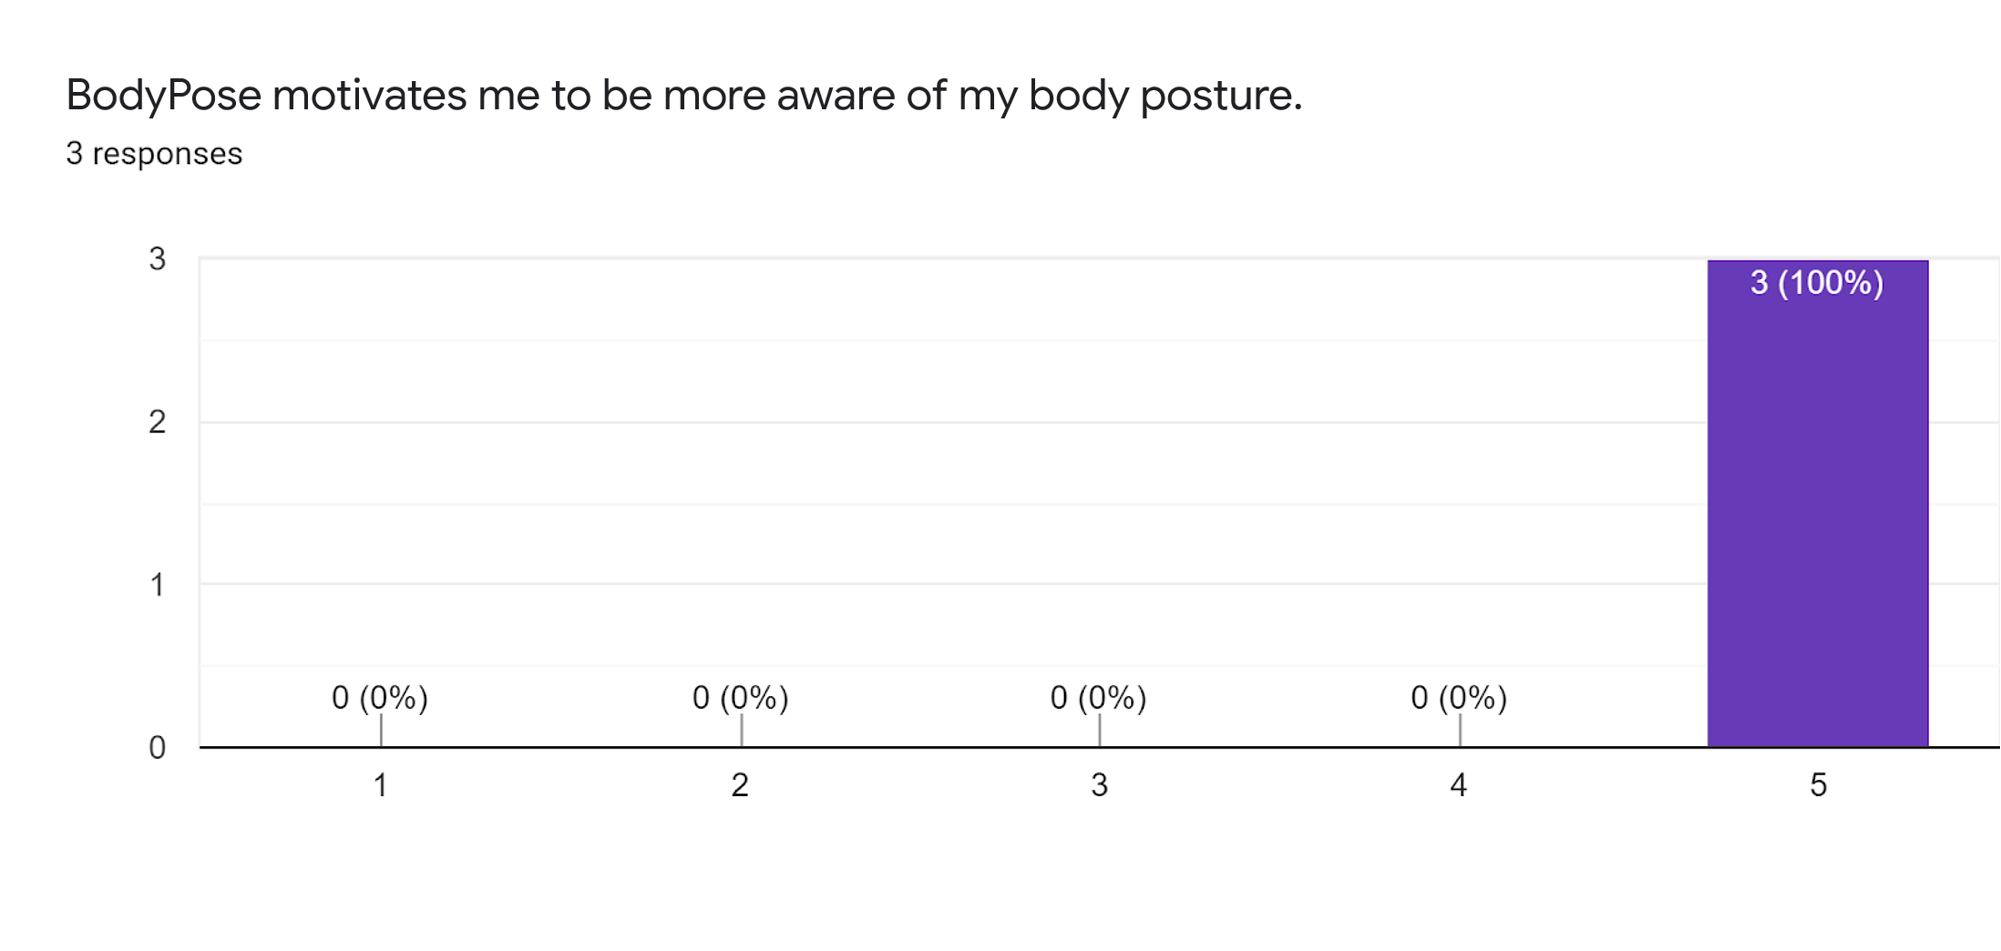
\includegraphics[width=0.32\textwidth]{media/us-gs-longterm-motivation-results-eng.png}
  }
  \subcaptionbox{Bar charts regarding workload, sense of control and creativity support\label{fig:ext-nasa-results}}{
    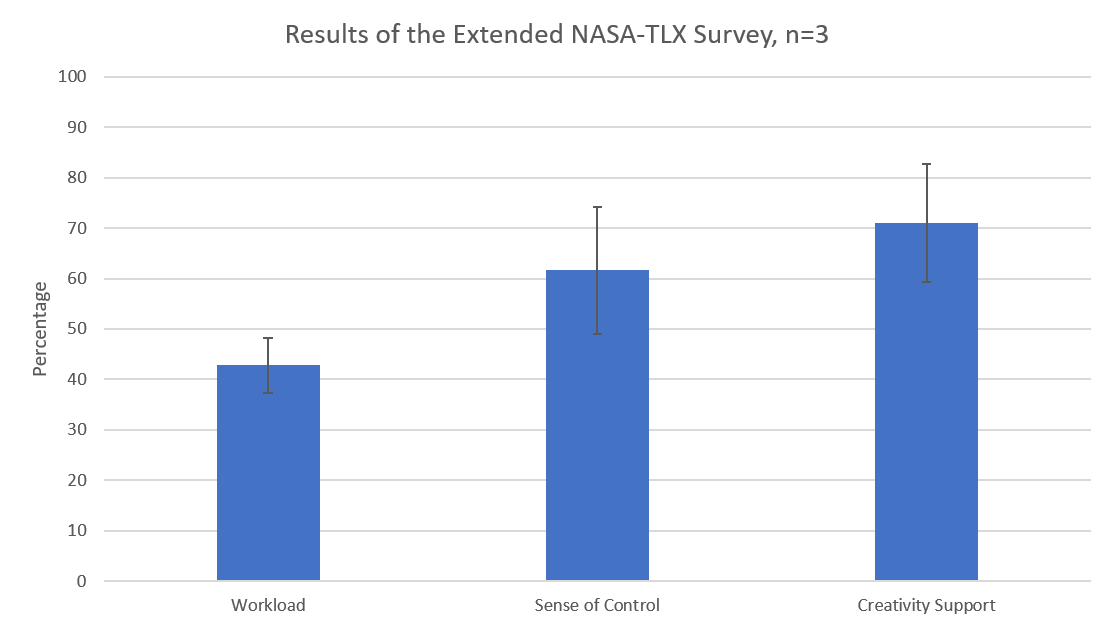
\includegraphics[width=0.32\textwidth]{media/us-ext-nasa-tlx-results.png}
  }
  \caption{User study measurements}
  \label{fig:measurements}
\end{figure*}

Users can stop monitoring by clicking on the corresponding stop button in the right end of the menu bar at the top of the page. In addition to the stop button, the menu bar offers a button to show the camera feed to the user, a button to enable/disable browser notifications and most importantly, a settings button. By clicking on the settings button, a settings menu will be shown on the right side of the screen, giving users the option to change the threshold values for the four measurement categories mentioned in \autoref{rulebased}, define the size of the window over which median or mean values are calculated, as well as set the time determining how long a bad posture needs to be held continuously before triggering a notification. Users may also choose between mean or median as a measure for central tendency, or to disable the so-called epoch mode altogether, i.e. keypoint data will not be aggregated, and only current real-time values are considered for evaluating a pose. Last but not least, users can download session data in the form of CSV tables. Data can be downloaded separately for different categories: users can choose from calibration data with respect to head or body, session data with respect to head or body, or a table containing all available information.

%%%
%%% User Study 1
%%%
\section{User Study} % in progress
\label{user-study-1}
We developed BodyPose as a reactive but accessible web application to detect slouching in computer-related work activities. To evaluate our approach, we conducted a user study in which we examined the effects of BodyPose on postural habits. Particularly, we were interested in measuring the user experience of BodyPose as well as its effect on short- and long-term motivation for correcting unhealthy postural misalignment. As BodyPose is intended to be used in workplace environments, we designed the tasks accordingly.

\subsection{Study Design}
\label{us1-study-design}
We used a within-groups study design (\autoref{fig:user-study-1}) in a controlled laboratory environment. Therefore, we controlled potential confounding variables such as workplace lighting, hardware and network stability.
The study focuses on gaining insights regarding user experience and motivational effects of BodyPose on maintaining or realigning to a healthy posture.\\
Evaluating user interfaces is not novel; therefore, we employed three commonly used metrics to evaluate BodyPose: the workload that a system provokes~\cite{hart1988development,hart2006nasa}, the creativity support that it provides~\cite{cherry2014quantifying} and the sense of control a user perceives~\cite{dong2015development}.

\subsection{Measurements}
\label{us1-measurements}
In order to measure the user experience and motivational effects, we used two questionnaires.
First, we designed a survey to gather quantitative personal information such as body height and weight as well as qualitative information referring to the participant's back pain history. We used this data to classify how severe the participants' back pain condition already is. Additionally, we included questions regarding the app's usability, various user interface impressions and the short- and long-term motivational impact of BodyPose. We used the 5-point Likert scale~\cite{likert1932technique} ($1=$Strongly disagree, $5=$Strongly agree).\\
Furthermore, we utilised an extended version of the NASA-TLX~\cite{hart2006nasa} to collect quantified data at the end of the tasks. The questionnaire measured workload, sense of control and creativity support. The Task-Load Index (TLX) from NASA~\cite{hart2006nasa} measured the subjective amount of workload experienced by the participants. The sense of control scale by Dong et al.~\cite{dong2015development}, adapted to a 20-point rating scale, measured perceived control. Finally, the Creativity Support Index by Cherry et al.~\cite{cherry2014quantifying}, limited to exploration, motivation and enjoyment dimensions, measured the creativity support.

\subsection{Study Tasks}
\label{us1-tasks}
We designed a set of two tasks to give the participants a chance to utilise the features of BodyPose. The first task gives the participants an overview of the features and encourages them to explore on their own. As BodyPose's intended area of the application lies in reactive background usage, task two simulates a work task and moves the app out of the visual scope of the screen.

\begin{description}
\item[Task A] This task consists of an introduction to the feature-set of BodyPose and encourages the participants to explore the user interface. The landing page of BodyPose explains the motivation and functionality of the app. Furthermore, it gives instructions on how to proceed. After browsing through the landing page, the instructions state the necessary steps of user actions to turn on BodyPose. After completing these steps, the participants executed a set of sub-tasks, including toggling the camera feed, as well as deactivating and reactivating the browser notifications. Finally, we instructed the participants to open the advanced settings drawer and experiment with various thresholds while observing possible changes and their effect on the app's operations.\\

\item[Task B]  In contrast to Task A, this task placed the website in the background and simulated a work task. We instructed the participants to write down their favourite recipe in a typical text program and to add a representative image from the internet. While performing this task, BodyPose was tracking the user from the background and gave feedback concerning the user's posture via browser notifications.
\end{description}

\subsection{Procedure}
\label{us1-procedure}
Ahead of the execution of the user study, we prepared three of our already tested devices by launching a browser with BodyPose and both questionnaires.
We instructed the participants to use BodyPose according to the tasks described in \autoref{us1-tasks} and to fill out the given survey consisting of the questionnaires described in \autoref{us1-measurements}. In order to keep the focus of the participants on exploring BodyPose freely, there were no time constraints given, as well as no signal when to proceed to the next task.
  

\subsection{Participants}
\label{us1-participants}
We recruited three participants (one female) for this user study. The median age was 24, with ages ranging from 23 to 27 years. Regarding the prior experience with back pain, 66\% of our participants reported that they had suffered from back pain at least once in their life. This is in line with the findings of \cite{osha2000facts}, reported in \autoref{introduction}.

\subsection{Data Analysis and Results}
\label{us1-data-analysis-results}
We changed the scale of the workload to 0-100 from 0-600 and the scale of creativity support to 0-100 from 0-300. Therefore the scales of our extended NASA-TLX regarding workload, control and creativity support were the same. The results of the extended NASA-TLX questionnaire, as shown in \autoref{fig:ext-nasa-results}, state that the participants rated the workload intensity at 43\%, with a standard deviation of 5,4\%. Furthermore, the participants rated sense of control during the task at 62\%, with a standard deviation of 13\%. Finally, they classified their subjective perception of creativity support at 71\%, with a standard deviation of 12\%.\\
Evaluating both questionnaires described in \autoref{us1-measurements}, the following insights were collected. First, \autoref{fig:us-gs-shortterm} states that all participants (100\%) strongly agreed that (on a short-term level) BodyPose motivated them to correct their body posture when being notified about an unhealthy alignment in their body posture.
Second, as the chart of \autoref{fig:us-gs-longterm} depicts, all (100\%) participants strongly agreed that BodyPose encourages them to become more aware of their body posture in the long-term.

\begin{figure}[htpb]
\centering
  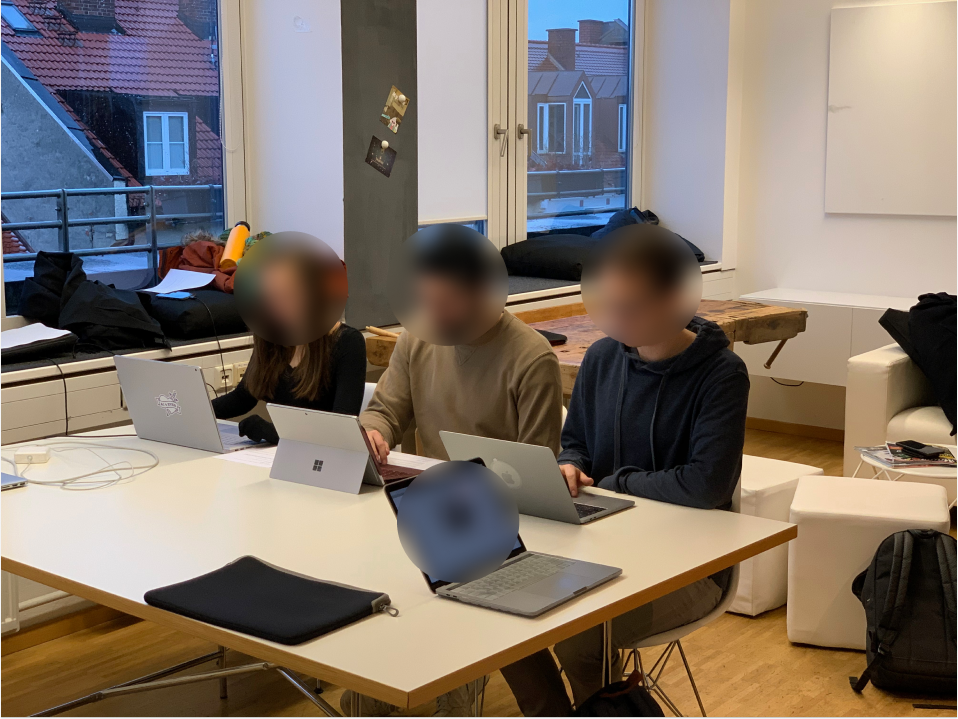
\includegraphics[width=\linewidth]{media/user-study-1.png}
  \caption{User study}
  \label{fig:user-study-1}
\end{figure}

% It should be noted, however, that this study is considered to be a test run. To gain reliable results and insights, a higher number of participants, as well as a more controlled and isolated setup, are required.

%\subsection{User Study Procedure}
%As only three participants took part in our user study, the results shown in \ref{us1-data-analysis-results} are statistically not representative. Furthermore, execution of the user study did not strictly follow the study protocol described in \ref{us1-procedure}: Since our participants were aware they were being observed not only by us but also by our mentors and colleagues, their behaviour might also not have been representative. Additionally, participants were not isolated from each other, so they did not perform their tasks independently. Lastly, since we recruited the participants from amongst our co-students, it can not be ruled out that personal bias(es) might have influenced the result.

%%%
%%% Discussion and future work
%%%
\section{Discussion and Future Work} % in progress
\label{discussion-future-work}

Our goal was to design, develop and evaluate BodyPose, a web app for body pose correction, offering feedback functionality with respect to unhealthy body poses in computer-related work activities. Additionally, our central premise consisted of offering an accessible solution, as well as being reactive, i.e. we only give feedback when necessary and credit pose correction attempts. 
Following our user study, we conclude that our rule-based feedback did achieve awareness concerning bad posture habits while working, as well as a strong consent throughout our participants concerning both its long- and short-term motivational feature to correct body posture. However, this outcome does not imply that this app yields health-related benefits in general; instead, it demonstrates that within the time frame available to us for this work, we were able to construct a working prototype with essential, yet limited functionality. Furthermore, we achieved a moderate workload, considerate sense of control and good creativity support on the user-end while handling the app. Overall, our approach seems feasible.\\ An apparent limitation is the absence of a status quo baseline, with which we could compare our collected data. However, the way in which we obtained data is easy to implement and thus reproducible without great effort.

There are several potential future avenues worth pursuing in order to enhance and improve the functionality of BodyPose. For instance, to allow for more personalised user experience, users should be able to create an account and save their preferences (such as threshold values). Furthermore, implementing a user identification system via face detection might prove helpful for robustness: Since BodyPose restricts the \textit{PoseNet} multi-pose detection algorithm to detecting only one pose per image, the system cannot handle situations robustly where multiple persons are visible to the camera. Identifying users with face detection would mitigate this problem, as the system can be modified only to evaluate the pose of a person who registered as a user. Another avenue for improving robustness, as well as accuracy, lies in replacing the pose detection model itself: \textit{PoseNet} detects two-dimensional poses (from two-dimensional input images), but some models can detect poses in three dimensions, even from two-dimensional input, such as in~\cite{Arnab_2019}. This model exhibits improved robustness and accuracy when compared to two-dimensional pose detection. However, due to the added complexity, further research concerning a potential performance trade-off is necessary. Furthermore, it would be interesting to test whether our rule-based system can be replaced by a machine learning model and if so, whether this leads to improved generalisation regarding the detection of poses (of different persons/in different settings). A last noteworthy potential avenue worth pursuing would be to extend the scope our application aims at: similar to ~\cite{jaimes2005sit}, detecting and monitoring user activities such as reading, typing, stretching could be used not only to give users feedback on how much time they spent for each activity during a session but also to give recommendations during a session to take a break or do some exercises.


%%%
%%% Conclusion
%%%
\section{Conclusion} % in progress
\label{conclusion}
We have presented a solution for helping computer users, especially workers, to correct bad body postures, maintain healthy body postures and improve body posture habits altogether. Due to the minimal setup requirements, our application is easily accessible and thus has the potential to reach a wide user-base: Anyone with a computer, a working internet connection and a webcam can use our application. Our test study shows that the application has the potential of motivating users successfully, both short-term and long-term: Users feel motivated by BodyPose to correct bad postures in the short-term, and to become more aware of their body posture habits in the long-term. However, a representative user study with more participants is required to confirm this potential, as well as to gain further insights not only into the workload, sense of control and creativity support as experienced by the user but also into accuracy, speed and robustness of our approach (when running on many different systems). Possible future avenues, as mentioned in \autoref{discussion-future-work}, bear the potential to improve robustness and accuracy, extend the scope and functionality of the application, and enhance the user experience.
% motivated users, both short-term and long-term


\appendix
%Appendix A
%\section{User Study 1: Visual search task}

%\begin{figure}[hbp]
%\centering
%\includegraphics[width=\linewidth]{media/us1.png}    
%\caption{Layer setup}
%\label{fig:us1layers}
%\end{figure}

\begin{acks} % in progress
  The authors would like to thank all three participants for their participation in the user study, as well as Dr Marco Meier, HYVE and TAWNY employees for their kind and helpful mentoring.
\end{acks}